\documentclass[twoside]{book}

% Packages required by doxygen
\usepackage{fixltx2e}
\usepackage{calc}
\usepackage{doxygen}
\usepackage[export]{adjustbox} % also loads graphicx
\usepackage{graphicx}
\usepackage[utf8]{inputenc}
\usepackage{makeidx}
\usepackage{multicol}
\usepackage{multirow}
\PassOptionsToPackage{warn}{textcomp}
\usepackage{textcomp}
\usepackage[nointegrals]{wasysym}
\usepackage[table]{xcolor}

% Font selection
\usepackage[T1]{fontenc}
\usepackage[scaled=.90]{helvet}
\usepackage{courier}
\usepackage{amssymb}
\usepackage{sectsty}
\renewcommand{\familydefault}{\sfdefault}
\allsectionsfont{%
  \fontseries{bc}\selectfont%
  \color{darkgray}%
}
\renewcommand{\DoxyLabelFont}{%
  \fontseries{bc}\selectfont%
  \color{darkgray}%
}
\newcommand{\+}{\discretionary{\mbox{\scriptsize$\hookleftarrow$}}{}{}}

% Page & text layout
\usepackage{geometry}
\geometry{%
  a4paper,%
  top=2.5cm,%
  bottom=2.5cm,%
  left=2.5cm,%
  right=2.5cm%
}
\tolerance=750
\hfuzz=15pt
\hbadness=750
\setlength{\emergencystretch}{15pt}
\setlength{\parindent}{0cm}
\setlength{\parskip}{3ex plus 2ex minus 2ex}
\makeatletter
\renewcommand{\paragraph}{%
  \@startsection{paragraph}{4}{0ex}{-1.0ex}{1.0ex}{%
    \normalfont\normalsize\bfseries\SS@parafont%
  }%
}
\renewcommand{\subparagraph}{%
  \@startsection{subparagraph}{5}{0ex}{-1.0ex}{1.0ex}{%
    \normalfont\normalsize\bfseries\SS@subparafont%
  }%
}
\makeatother

% Headers & footers
\usepackage{fancyhdr}
\pagestyle{fancyplain}
\fancyhead[LE]{\fancyplain{}{\bfseries\thepage}}
\fancyhead[CE]{\fancyplain{}{}}
\fancyhead[RE]{\fancyplain{}{\bfseries\leftmark}}
\fancyhead[LO]{\fancyplain{}{\bfseries\rightmark}}
\fancyhead[CO]{\fancyplain{}{}}
\fancyhead[RO]{\fancyplain{}{\bfseries\thepage}}
\fancyfoot[LE]{\fancyplain{}{}}
\fancyfoot[CE]{\fancyplain{}{}}
\fancyfoot[RE]{\fancyplain{}{\bfseries\scriptsize Generated by Doxygen }}
\fancyfoot[LO]{\fancyplain{}{\bfseries\scriptsize Generated by Doxygen }}
\fancyfoot[CO]{\fancyplain{}{}}
\fancyfoot[RO]{\fancyplain{}{}}
\renewcommand{\footrulewidth}{0.4pt}
\renewcommand{\chaptermark}[1]{%
  \markboth{#1}{}%
}
\renewcommand{\sectionmark}[1]{%
  \markright{\thesection\ #1}%
}

% Indices & bibliography
\usepackage{natbib}
\usepackage[titles]{tocloft}
\setcounter{tocdepth}{3}
\setcounter{secnumdepth}{5}
\makeindex

% Hyperlinks (required, but should be loaded last)
\usepackage{ifpdf}
\ifpdf
  \usepackage[pdftex,pagebackref=true]{hyperref}
\else
  \usepackage[ps2pdf,pagebackref=true]{hyperref}
\fi
\hypersetup{%
  colorlinks=true,%
  linkcolor=blue,%
  citecolor=blue,%
  unicode%
}

% Custom commands
\newcommand{\clearemptydoublepage}{%
  \newpage{\pagestyle{empty}\cleardoublepage}%
}

\usepackage{caption}
\captionsetup{labelsep=space,justification=centering,font={bf},singlelinecheck=off,skip=4pt,position=top}

%===== C O N T E N T S =====

\begin{document}

% Titlepage & ToC
\hypersetup{pageanchor=false,
             bookmarksnumbered=true,
             pdfencoding=unicode
            }
\pagenumbering{alph}
\begin{titlepage}
\vspace*{7cm}
\begin{center}%
{\Large My Project }\\
\vspace*{1cm}
{\large Generated by Doxygen 1.8.15}\\
\end{center}
\end{titlepage}
\clearemptydoublepage
\pagenumbering{roman}
\tableofcontents
\clearemptydoublepage
\pagenumbering{arabic}
\hypersetup{pageanchor=true}

%--- Begin generated contents ---
\chapter{Hierarchical Index}
\section{Class Hierarchy}
This inheritance list is sorted roughly, but not completely, alphabetically\+:\begin{DoxyCompactList}
\item \contentsline{section}{circulo}{\pageref{classcirculo}}{}
\item \contentsline{section}{cubo}{\pageref{classcubo}}{}
\item \contentsline{section}{esfera}{\pageref{classesfera}}{}
\item \contentsline{section}{geometria}{\pageref{classgeometria}}{}
\item \contentsline{section}{paralelepipedo}{\pageref{classparalelepipedo}}{}
\item \contentsline{section}{piramide}{\pageref{classpiramide}}{}
\item \contentsline{section}{quadrado}{\pageref{classquadrado}}{}
\item \contentsline{section}{retangulo}{\pageref{classretangulo}}{}
\item \contentsline{section}{triangulo}{\pageref{classtriangulo}}{}
\item exception\begin{DoxyCompactList}
\item \contentsline{section}{Argumentos\+Errados}{\pageref{classArgumentosErrados}}{}
\item \contentsline{section}{Figura\+Nao\+Cadastrada}{\pageref{classFiguraNaoCadastrada}}{}
\item \contentsline{section}{Number}{\pageref{classNumber}}{}
\end{DoxyCompactList}
\end{DoxyCompactList}

\chapter{Class Index}
\section{Class List}
Here are the classes, structs, unions and interfaces with brief descriptions\+:\begin{DoxyCompactList}
\item\contentsline{section}{\mbox{\hyperlink{classbanco}{banco}} }{\pageref{classbanco}}{}
\item\contentsline{section}{\mbox{\hyperlink{classconta}{conta}} }{\pageref{classconta}}{}
\item\contentsline{section}{\mbox{\hyperlink{classcontaCorrente}{conta\+Corrente}} }{\pageref{classcontaCorrente}}{}
\item\contentsline{section}{\mbox{\hyperlink{classcontaPoupanca}{conta\+Poupanca}} }{\pageref{classcontaPoupanca}}{}
\item\contentsline{section}{\mbox{\hyperlink{classmovimentacao}{movimentacao}} }{\pageref{classmovimentacao}}{}
\end{DoxyCompactList}

\chapter{Class Documentation}
\hypertarget{classArgumentosErrados}{}\section{Argumentos\+Errados Class Reference}
\label{classArgumentosErrados}\index{Argumentos\+Errados@{Argumentos\+Errados}}


{\ttfamily \#include $<$excecao.\+h$>$}

Inheritance diagram for Argumentos\+Errados\+:\begin{figure}[H]
\begin{center}
\leavevmode
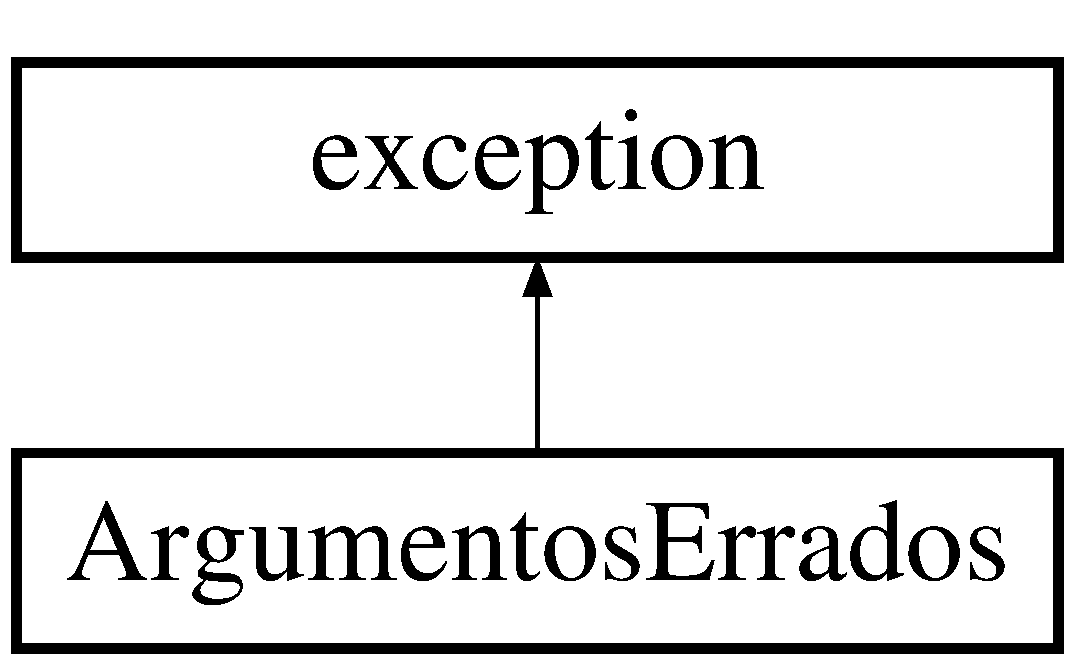
\includegraphics[height=2.000000cm]{classArgumentosErrados}
\end{center}
\end{figure}
\subsection*{Public Member Functions}
\begin{DoxyCompactItemize}
\item 
\mbox{\Hypertarget{classArgumentosErrados_a9d23e10092cd69f8e9fdc94074a24ecf}\label{classArgumentosErrados_a9d23e10092cd69f8e9fdc94074a24ecf}} 
const char $\ast$ {\bfseries what} ()
\end{DoxyCompactItemize}


\subsection{Detailed Description}
Argumentos inválidos. 

The documentation for this class was generated from the following file\+:\begin{DoxyCompactItemize}
\item 
excecao.\+h\end{DoxyCompactItemize}

\hypertarget{classcirculo}{}\section{circulo Class Reference}
\label{classcirculo}\index{circulo@{circulo}}
\subsection*{Public Member Functions}
\begin{DoxyCompactItemize}
\item 
\mbox{\Hypertarget{classcirculo_adb9dc9e9ad1c10bc0d2f69d08d04339b}\label{classcirculo_adb9dc9e9ad1c10bc0d2f69d08d04339b}} 
{\bfseries circulo} (float Raio)
\item 
\mbox{\Hypertarget{classcirculo_a3c137b5efd621252e95c1db378eb2cd6}\label{classcirculo_a3c137b5efd621252e95c1db378eb2cd6}} 
float {\bfseries get\+Area} ()
\item 
\mbox{\Hypertarget{classcirculo_aa8547bc9d38318b6c5ba40160514d0d5}\label{classcirculo_aa8547bc9d38318b6c5ba40160514d0d5}} 
float {\bfseries get\+Perimetro} ()
\end{DoxyCompactItemize}


The documentation for this class was generated from the following files\+:\begin{DoxyCompactItemize}
\item 
circulo.\+h\item 
circulo.\+cpp\end{DoxyCompactItemize}

\hypertarget{classcubo}{}\section{cubo Class Reference}
\label{classcubo}\index{cubo@{cubo}}
\subsection*{Public Member Functions}
\begin{DoxyCompactItemize}
\item 
\mbox{\Hypertarget{classcubo_a4dd22a35efe95be848258e049c93585d}\label{classcubo_a4dd22a35efe95be848258e049c93585d}} 
{\bfseries cubo} (float Aresta)
\item 
\mbox{\Hypertarget{classcubo_a593b69876efbbf1e2f9ca70e927913de}\label{classcubo_a593b69876efbbf1e2f9ca70e927913de}} 
float {\bfseries get\+Volume} ()
\item 
\mbox{\Hypertarget{classcubo_ac00b5f188051f12f591b68c923f03c6a}\label{classcubo_ac00b5f188051f12f591b68c923f03c6a}} 
float {\bfseries get\+Area} ()
\end{DoxyCompactItemize}


The documentation for this class was generated from the following files\+:\begin{DoxyCompactItemize}
\item 
cubo.\+h\item 
cubo.\+cpp\end{DoxyCompactItemize}

\hypertarget{classesfera}{}\section{esfera Class Reference}
\label{classesfera}\index{esfera@{esfera}}
\subsection*{Public Member Functions}
\begin{DoxyCompactItemize}
\item 
\mbox{\Hypertarget{classesfera_a762e1a57578e9e8097c5191bd5b237a6}\label{classesfera_a762e1a57578e9e8097c5191bd5b237a6}} 
{\bfseries esfera} (float Raio)
\item 
\mbox{\Hypertarget{classesfera_a19e30591416ffb5ae58df613950f0ee7}\label{classesfera_a19e30591416ffb5ae58df613950f0ee7}} 
float {\bfseries get\+Area} ()
\item 
\mbox{\Hypertarget{classesfera_a8b0c9091d027eef8d17a3583058eefbb}\label{classesfera_a8b0c9091d027eef8d17a3583058eefbb}} 
float {\bfseries get\+Volume} ()
\end{DoxyCompactItemize}


The documentation for this class was generated from the following files\+:\begin{DoxyCompactItemize}
\item 
esfera.\+h\item 
esfera.\+cpp\end{DoxyCompactItemize}

\hypertarget{classFiguraNaoCadastrada}{}\section{Figura\+Nao\+Cadastrada Class Reference}
\label{classFiguraNaoCadastrada}\index{Figura\+Nao\+Cadastrada@{Figura\+Nao\+Cadastrada}}


{\ttfamily \#include $<$excecao.\+h$>$}

Inheritance diagram for Figura\+Nao\+Cadastrada\+:\begin{figure}[H]
\begin{center}
\leavevmode
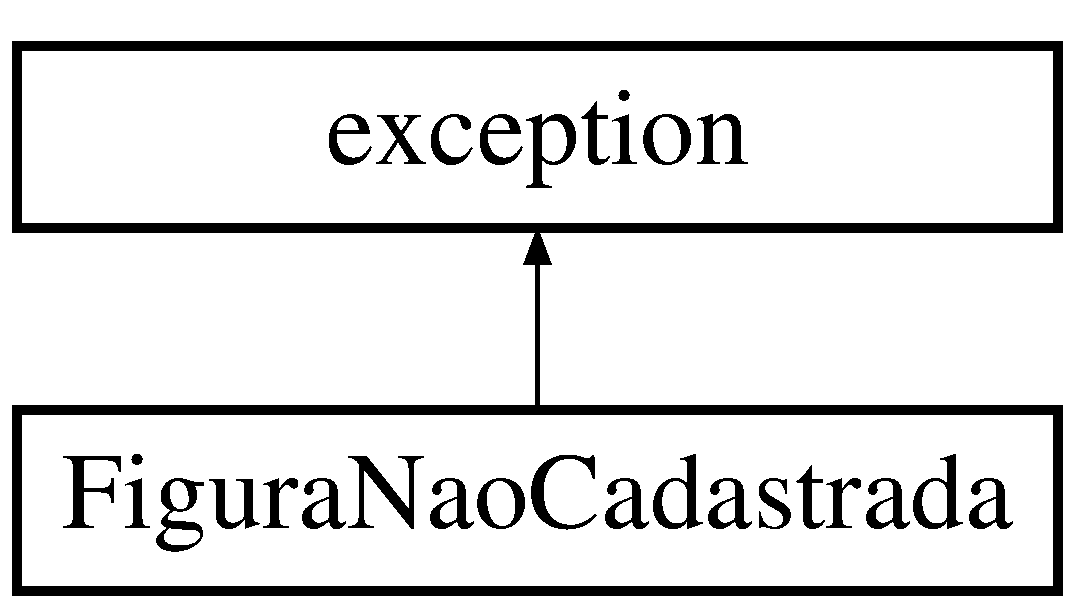
\includegraphics[height=2.000000cm]{classFiguraNaoCadastrada}
\end{center}
\end{figure}
\subsection*{Public Member Functions}
\begin{DoxyCompactItemize}
\item 
\mbox{\Hypertarget{classFiguraNaoCadastrada_a1ed08ee074df9180eafca07728e2b455}\label{classFiguraNaoCadastrada_a1ed08ee074df9180eafca07728e2b455}} 
const char $\ast$ {\bfseries what} ()
\end{DoxyCompactItemize}


\subsection{Detailed Description}
Figura não cadastrada no banco de dados. 

The documentation for this class was generated from the following file\+:\begin{DoxyCompactItemize}
\item 
excecao.\+h\end{DoxyCompactItemize}

\hypertarget{classgeometria}{}\section{geometria Class Reference}
\label{classgeometria}\index{geometria@{geometria}}
\subsection*{Public Member Functions}
\begin{DoxyCompactItemize}
\item 
\mbox{\Hypertarget{classgeometria_a1ec5a89280795e3c16039e78e1c79d9b}\label{classgeometria_a1ec5a89280795e3c16039e78e1c79d9b}} 
{\bfseries geometria} (std\+::vector$<$ std\+::string $>$ a)
\item 
void \mbox{\hyperlink{classgeometria_a8d79ad08a59914d895f22a2e08269ca9}{redirecionar}} ()
\item 
void \mbox{\hyperlink{classgeometria_a6c4f67cda5e77a099232bdd5b9ff2df9}{exibir\+Lista}} ()
\end{DoxyCompactItemize}


\subsection{Member Function Documentation}
\mbox{\Hypertarget{classgeometria_a6c4f67cda5e77a099232bdd5b9ff2df9}\label{classgeometria_a6c4f67cda5e77a099232bdd5b9ff2df9}} 
\index{geometria@{geometria}!exibir\+Lista@{exibir\+Lista}}
\index{exibir\+Lista@{exibir\+Lista}!geometria@{geometria}}
\subsubsection{\texorpdfstring{exibir\+Lista()}{exibirLista()}}
{\footnotesize\ttfamily void geometria\+::exibir\+Lista (\begin{DoxyParamCaption}{ }\end{DoxyParamCaption})}

lista de comandos para auxiliar o usuário.\mbox{\Hypertarget{classgeometria_a8d79ad08a59914d895f22a2e08269ca9}\label{classgeometria_a8d79ad08a59914d895f22a2e08269ca9}} 
\index{geometria@{geometria}!redirecionar@{redirecionar}}
\index{redirecionar@{redirecionar}!geometria@{geometria}}
\subsubsection{\texorpdfstring{redirecionar()}{redirecionar()}}
{\footnotesize\ttfamily void geometria\+::redirecionar (\begin{DoxyParamCaption}{ }\end{DoxyParamCaption})}

Compara a primeira posição do vector com a auxiliar para entrar na classe apropriada.

Ajusta-\/se o tamanho do comparador com a quantidade de membros da classe para evitar falhas de segmentação. \begin{DoxyReturn}{Returns}
Os dados da figura geométrica ou em caso de erro a lista de dados.
\end{DoxyReturn}
Verifica se o tamanho dos dados batem com a especificações da figura, presente em todas as figuras.

The documentation for this class was generated from the following files\+:\begin{DoxyCompactItemize}
\item 
geometria.\+h\item 
geometria.\+cpp\end{DoxyCompactItemize}

\hypertarget{classNumber}{}\section{Number Class Reference}
\label{classNumber}\index{Number@{Number}}


{\ttfamily \#include $<$excecao.\+h$>$}

Inheritance diagram for Number\+:\begin{figure}[H]
\begin{center}
\leavevmode
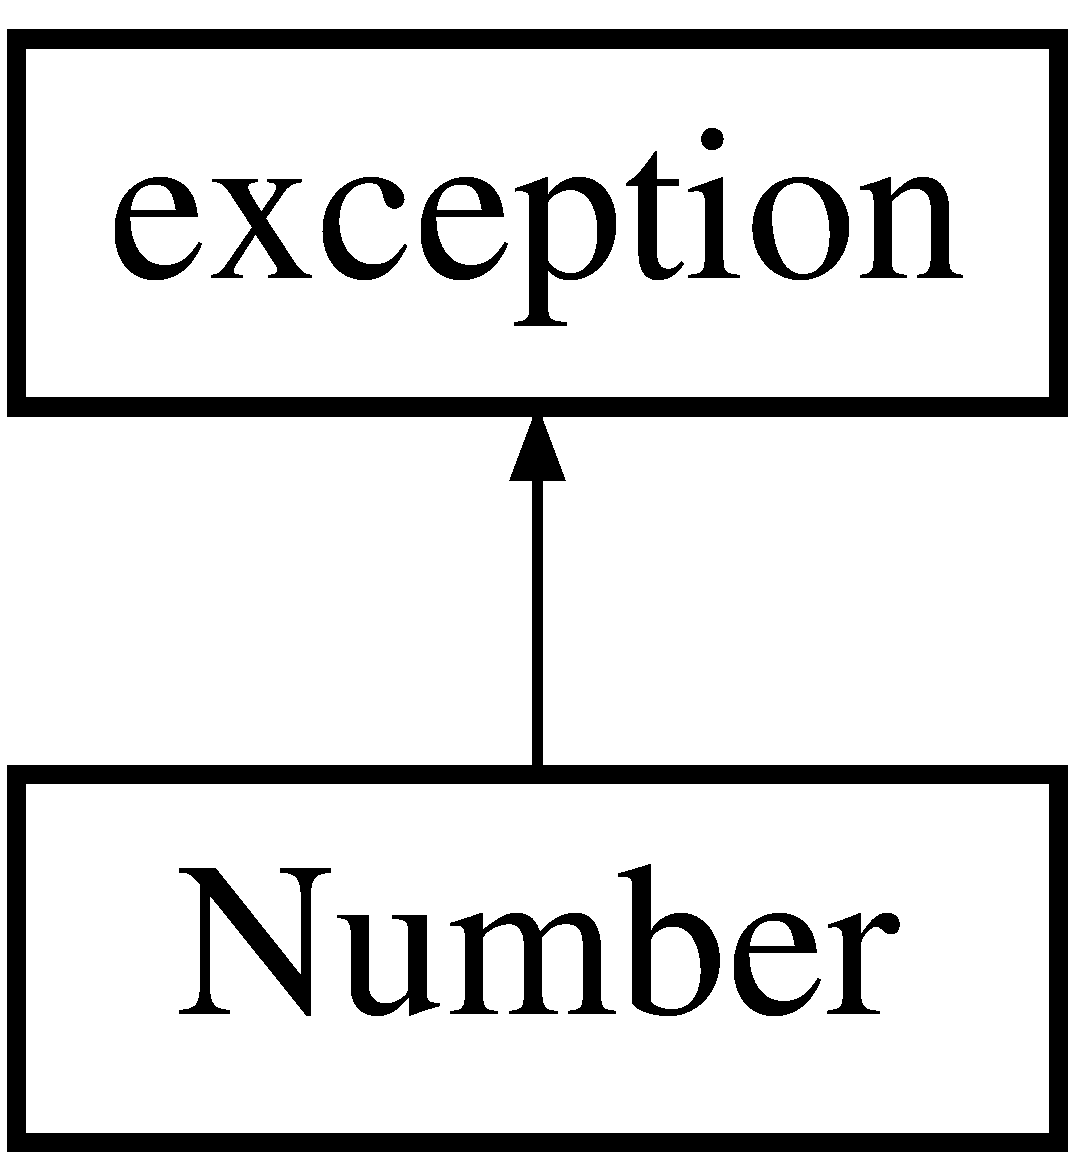
\includegraphics[height=2.000000cm]{classNumber}
\end{center}
\end{figure}
\subsection*{Public Member Functions}
\begin{DoxyCompactItemize}
\item 
\mbox{\Hypertarget{classNumber_addefb1064a86bcd1db99b1a38bd730ac}\label{classNumber_addefb1064a86bcd1db99b1a38bd730ac}} 
const char $\ast$ {\bfseries what} ()
\end{DoxyCompactItemize}


\subsection{Detailed Description}
Número negativo ou zero. 

The documentation for this class was generated from the following file\+:\begin{DoxyCompactItemize}
\item 
excecao.\+h\end{DoxyCompactItemize}

\hypertarget{classparalelepipedo}{}\section{paralelepipedo Class Reference}
\label{classparalelepipedo}\index{paralelepipedo@{paralelepipedo}}
\subsection*{Public Member Functions}
\begin{DoxyCompactItemize}
\item 
\mbox{\Hypertarget{classparalelepipedo_a6e79667bf9e689881ac538f9eb7d558a}\label{classparalelepipedo_a6e79667bf9e689881ac538f9eb7d558a}} 
{\bfseries paralelepipedo} (float Aresta1, float Aresta2, float Aresta3)
\item 
\mbox{\Hypertarget{classparalelepipedo_a10c9308080ebd3e8e0dc68183111b272}\label{classparalelepipedo_a10c9308080ebd3e8e0dc68183111b272}} 
float {\bfseries get\+Area} ()
\item 
\mbox{\Hypertarget{classparalelepipedo_af79e9fe7f95661e7747dd5d233c564fb}\label{classparalelepipedo_af79e9fe7f95661e7747dd5d233c564fb}} 
float {\bfseries get\+Volume} ()
\end{DoxyCompactItemize}


The documentation for this class was generated from the following files\+:\begin{DoxyCompactItemize}
\item 
paralelepipedo.\+h\item 
paralelepipedo.\+cpp\end{DoxyCompactItemize}

\hypertarget{classpiramide}{}\section{piramide Class Reference}
\label{classpiramide}\index{piramide@{piramide}}
\subsection*{Public Member Functions}
\begin{DoxyCompactItemize}
\item 
\mbox{\hyperlink{classpiramide_a095873f62dcf579692142be456c1bbb6}{piramide}} (float base\+Triangulo, float altura\+Triangulo, float lado\+Quadrado, float Altura\+Piramide)
\begin{DoxyCompactList}\small\item\em Usa métodos da classe quadrado e triângulo para definições. \end{DoxyCompactList}\item 
\mbox{\Hypertarget{classpiramide_a1ca04b666b157a3e5c74206e7eacc5ed}\label{classpiramide_a1ca04b666b157a3e5c74206e7eacc5ed}} 
float {\bfseries get\+Area} ()
\item 
\mbox{\Hypertarget{classpiramide_ad003a47e0de28eb2ae2b7ff638460e1b}\label{classpiramide_ad003a47e0de28eb2ae2b7ff638460e1b}} 
float {\bfseries get\+Volume} ()
\end{DoxyCompactItemize}


\subsection{Constructor \& Destructor Documentation}
\mbox{\Hypertarget{classpiramide_a095873f62dcf579692142be456c1bbb6}\label{classpiramide_a095873f62dcf579692142be456c1bbb6}} 
\index{piramide@{piramide}!piramide@{piramide}}
\index{piramide@{piramide}!piramide@{piramide}}
\subsubsection{\texorpdfstring{piramide()}{piramide()}}
{\footnotesize\ttfamily piramide\+::piramide (\begin{DoxyParamCaption}\item[{float}]{base\+Triangulo,  }\item[{float}]{altura\+Triangulo,  }\item[{float}]{lado\+Quadrado,  }\item[{float}]{Altura\+Piramide }\end{DoxyParamCaption})}



Usa métodos da classe quadrado e triângulo para definições. 


\begin{DoxyParams}{Parameters}
{\em recebe-\/se} & base triângulo, altura do triângulo, lado do quadrado e altura da pirâmide \\
\hline
\end{DoxyParams}


The documentation for this class was generated from the following files\+:\begin{DoxyCompactItemize}
\item 
piramide.\+h\item 
piramide.\+cpp\end{DoxyCompactItemize}

\hypertarget{classquadrado}{}\section{quadrado Class Reference}
\label{classquadrado}\index{quadrado@{quadrado}}
\subsection*{Public Member Functions}
\begin{DoxyCompactItemize}
\item 
\mbox{\Hypertarget{classquadrado_a78da6b808ea4202775c7b7636f12fba3}\label{classquadrado_a78da6b808ea4202775c7b7636f12fba3}} 
{\bfseries quadrado} (float Lado)
\item 
\mbox{\Hypertarget{classquadrado_a2e56c1ddbf3605d533b0635e1f5b4de4}\label{classquadrado_a2e56c1ddbf3605d533b0635e1f5b4de4}} 
float {\bfseries get\+Perimetro} ()
\item 
\mbox{\Hypertarget{classquadrado_a1853ba2eb28b1926698f8d2a228cda78}\label{classquadrado_a1853ba2eb28b1926698f8d2a228cda78}} 
float {\bfseries get\+Area} ()
\end{DoxyCompactItemize}


The documentation for this class was generated from the following files\+:\begin{DoxyCompactItemize}
\item 
quadrado.\+h\item 
quadrado.\+cpp\end{DoxyCompactItemize}

\hypertarget{classretangulo}{}\section{retangulo Class Reference}
\label{classretangulo}\index{retangulo@{retangulo}}
\subsection*{Public Member Functions}
\begin{DoxyCompactItemize}
\item 
\mbox{\Hypertarget{classretangulo_a73af5a662bc6e654c7507ba72cfcb618}\label{classretangulo_a73af5a662bc6e654c7507ba72cfcb618}} 
{\bfseries retangulo} (float Base, float Altura)
\item 
\mbox{\Hypertarget{classretangulo_a4179fe202f792944875044f1853f16bf}\label{classretangulo_a4179fe202f792944875044f1853f16bf}} 
float {\bfseries get\+Perimetro} ()
\item 
\mbox{\Hypertarget{classretangulo_a19ac519a86f37f6dfb460cbfd4e6004b}\label{classretangulo_a19ac519a86f37f6dfb460cbfd4e6004b}} 
float {\bfseries get\+Area} ()
\end{DoxyCompactItemize}


The documentation for this class was generated from the following files\+:\begin{DoxyCompactItemize}
\item 
retangulo.\+h\item 
retangulo.\+cpp\end{DoxyCompactItemize}

\hypertarget{classtriangulo}{}\section{triangulo Class Reference}
\label{classtriangulo}\index{triangulo@{triangulo}}
\subsection*{Public Member Functions}
\begin{DoxyCompactItemize}
\item 
\mbox{\Hypertarget{classtriangulo_ae0fc3ebd92250ab83327de75c474fd98}\label{classtriangulo_ae0fc3ebd92250ab83327de75c474fd98}} 
{\bfseries triangulo} (float Base, float Altura)
\item 
\mbox{\Hypertarget{classtriangulo_a473de9df3b8888c11d430ad2797024d8}\label{classtriangulo_a473de9df3b8888c11d430ad2797024d8}} 
float {\bfseries get\+Perimetro} ()
\item 
\mbox{\Hypertarget{classtriangulo_a9e0460d41e519fc931735f4ed2811b37}\label{classtriangulo_a9e0460d41e519fc931735f4ed2811b37}} 
float {\bfseries get\+Area} ()
\end{DoxyCompactItemize}


The documentation for this class was generated from the following files\+:\begin{DoxyCompactItemize}
\item 
triangulo.\+h\item 
triangulo.\+cpp\end{DoxyCompactItemize}

%--- End generated contents ---

% Index
\backmatter
\newpage
\phantomsection
\clearemptydoublepage
\addcontentsline{toc}{chapter}{\indexname}
\printindex

\end{document}
